\documentclass[twoside,11pt]{article}

% Any additional packages needed should be included after jmlr2e.
% Note that jmlr2e.sty includes epsfig, amssymb, natbib and graphicx,
% and defines many common macros, such as 'proof' and 'example'.
%
% It also sets the bibliographystyle to plainnat; for more information on
% natbib citation styles, see the natbib documentation, a copy of which
% is archived at http://www.jmlr.org/format/natbib.pdf

\usepackage{jmlr2e}
\usepackage{multirow}
\usepackage{booktabs}
\usepackage{xspace}
\usepackage{graphicx}
\usepackage{subfig}
\usepackage[inline]{enumitem}
\usepackage{hyperref}
\usepackage{amsmath,amsfonts,dsfont,mathrsfs,mathtools,amssymb}
\usepackage{algorithm, algpseudocode}

\usepackage{fancyvrb}
\usepackage{color}
\usepackage[utf8]{inputenc}


\makeatletter
\def\PY@reset{\let\PY@it=\relax \let\PY@bf=\relax%
    \let\PY@ul=\relax \let\PY@tc=\relax%
    \let\PY@bc=\relax \let\PY@ff=\relax}
\def\PY@tok#1{\csname PY@tok@#1\endcsname}
\def\PY@toks#1+{\ifx\relax#1\empty\else%
    \PY@tok{#1}\expandafter\PY@toks\fi}
\def\PY@do#1{\PY@bc{\PY@tc{\PY@ul{%
    \PY@it{\PY@bf{\PY@ff{#1}}}}}}}
\def\PY#1#2{\PY@reset\PY@toks#1+\relax+\PY@do{#2}}

\expandafter\def\csname PY@tok@se\endcsname{\let\PY@bf=\textbf\def\PY@tc##1{\textcolor[rgb]{0.73,0.40,0.13}{##1}}}
\expandafter\def\csname PY@tok@kp\endcsname{\def\PY@tc##1{\textcolor[rgb]{0.67,0.13,1.00}{##1}}}
\expandafter\def\csname PY@tok@il\endcsname{\def\PY@tc##1{\textcolor[rgb]{0.40,0.40,0.40}{##1}}}
\expandafter\def\csname PY@tok@cm\endcsname{\let\PY@it=\textit\def\PY@tc##1{\textcolor[rgb]{0.00,0.53,0.00}{##1}}}
\expandafter\def\csname PY@tok@ow\endcsname{\let\PY@bf=\textbf\def\PY@tc##1{\textcolor[rgb]{0.67,0.13,1.00}{##1}}}
\expandafter\def\csname PY@tok@nn\endcsname{\let\PY@bf=\textbf\def\PY@tc##1{\textcolor[rgb]{0.00,0.00,1.00}{##1}}}
\expandafter\def\csname PY@tok@gd\endcsname{\def\PY@tc##1{\textcolor[rgb]{0.63,0.00,0.00}{##1}}}
\expandafter\def\csname PY@tok@kr\endcsname{\let\PY@bf=\textbf\def\PY@tc##1{\textcolor[rgb]{0.67,0.13,1.00}{##1}}}
\expandafter\def\csname PY@tok@cpf\endcsname{\let\PY@it=\textit\def\PY@tc##1{\textcolor[rgb]{0.00,0.53,0.00}{##1}}}
\expandafter\def\csname PY@tok@gt\endcsname{\def\PY@tc##1{\textcolor[rgb]{0.00,0.27,0.87}{##1}}}
\expandafter\def\csname PY@tok@gh\endcsname{\let\PY@bf=\textbf\def\PY@tc##1{\textcolor[rgb]{0.00,0.00,0.50}{##1}}}
\expandafter\def\csname PY@tok@c\endcsname{\let\PY@it=\textit\def\PY@tc##1{\textcolor[rgb]{0.00,0.53,0.00}{##1}}}
\expandafter\def\csname PY@tok@s2\endcsname{\def\PY@tc##1{\textcolor[rgb]{0.73,0.27,0.27}{##1}}}
\expandafter\def\csname PY@tok@gp\endcsname{\let\PY@bf=\textbf\def\PY@tc##1{\textcolor[rgb]{0.00,0.00,0.50}{##1}}}
\expandafter\def\csname PY@tok@ge\endcsname{\let\PY@it=\textit}
\expandafter\def\csname PY@tok@na\endcsname{\def\PY@tc##1{\textcolor[rgb]{0.73,0.27,0.27}{##1}}}
\expandafter\def\csname PY@tok@gi\endcsname{\def\PY@tc##1{\textcolor[rgb]{0.00,0.63,0.00}{##1}}}
\expandafter\def\csname PY@tok@mb\endcsname{\def\PY@tc##1{\textcolor[rgb]{0.40,0.40,0.40}{##1}}}
\expandafter\def\csname PY@tok@ch\endcsname{\let\PY@it=\textit\def\PY@tc##1{\textcolor[rgb]{0.00,0.53,0.00}{##1}}}
\expandafter\def\csname PY@tok@kc\endcsname{\let\PY@bf=\textbf\def\PY@tc##1{\textcolor[rgb]{0.67,0.13,1.00}{##1}}}
\expandafter\def\csname PY@tok@kd\endcsname{\let\PY@bf=\textbf\def\PY@tc##1{\textcolor[rgb]{0.67,0.13,1.00}{##1}}}
\expandafter\def\csname PY@tok@no\endcsname{\def\PY@tc##1{\textcolor[rgb]{0.53,0.00,0.00}{##1}}}
\expandafter\def\csname PY@tok@s\endcsname{\def\PY@tc##1{\textcolor[rgb]{0.73,0.27,0.27}{##1}}}
\expandafter\def\csname PY@tok@kn\endcsname{\let\PY@bf=\textbf\def\PY@tc##1{\textcolor[rgb]{0.67,0.13,1.00}{##1}}}
\expandafter\def\csname PY@tok@vg\endcsname{\def\PY@tc##1{\textcolor[rgb]{0.72,0.53,0.04}{##1}}}
\expandafter\def\csname PY@tok@vi\endcsname{\def\PY@tc##1{\textcolor[rgb]{0.72,0.53,0.04}{##1}}}
\expandafter\def\csname PY@tok@mo\endcsname{\def\PY@tc##1{\textcolor[rgb]{0.40,0.40,0.40}{##1}}}
\expandafter\def\csname PY@tok@sr\endcsname{\def\PY@tc##1{\textcolor[rgb]{0.73,0.40,0.53}{##1}}}
\expandafter\def\csname PY@tok@cs\endcsname{\let\PY@bf=\textbf\def\PY@tc##1{\textcolor[rgb]{0.00,0.53,0.00}{##1}}}
\expandafter\def\csname PY@tok@mh\endcsname{\def\PY@tc##1{\textcolor[rgb]{0.40,0.40,0.40}{##1}}}
\expandafter\def\csname PY@tok@ss\endcsname{\def\PY@tc##1{\textcolor[rgb]{0.72,0.53,0.04}{##1}}}
\expandafter\def\csname PY@tok@nb\endcsname{\def\PY@tc##1{\textcolor[rgb]{0.67,0.13,1.00}{##1}}}
\expandafter\def\csname PY@tok@sx\endcsname{\def\PY@tc##1{\textcolor[rgb]{0.00,0.50,0.00}{##1}}}
\expandafter\def\csname PY@tok@sb\endcsname{\def\PY@tc##1{\textcolor[rgb]{0.73,0.27,0.27}{##1}}}
\expandafter\def\csname PY@tok@mi\endcsname{\def\PY@tc##1{\textcolor[rgb]{0.40,0.40,0.40}{##1}}}
\expandafter\def\csname PY@tok@si\endcsname{\let\PY@bf=\textbf\def\PY@tc##1{\textcolor[rgb]{0.73,0.40,0.53}{##1}}}
\expandafter\def\csname PY@tok@s1\endcsname{\def\PY@tc##1{\textcolor[rgb]{0.73,0.27,0.27}{##1}}}
\expandafter\def\csname PY@tok@gu\endcsname{\let\PY@bf=\textbf\def\PY@tc##1{\textcolor[rgb]{0.50,0.00,0.50}{##1}}}
\expandafter\def\csname PY@tok@nt\endcsname{\let\PY@bf=\textbf\def\PY@tc##1{\textcolor[rgb]{0.00,0.50,0.00}{##1}}}
\expandafter\def\csname PY@tok@vc\endcsname{\def\PY@tc##1{\textcolor[rgb]{0.72,0.53,0.04}{##1}}}
\expandafter\def\csname PY@tok@ni\endcsname{\let\PY@bf=\textbf\def\PY@tc##1{\textcolor[rgb]{0.60,0.60,0.60}{##1}}}
\expandafter\def\csname PY@tok@sc\endcsname{\def\PY@tc##1{\textcolor[rgb]{0.73,0.27,0.27}{##1}}}
\expandafter\def\csname PY@tok@ne\endcsname{\let\PY@bf=\textbf\def\PY@tc##1{\textcolor[rgb]{0.82,0.25,0.23}{##1}}}
\expandafter\def\csname PY@tok@c1\endcsname{\let\PY@it=\textit\def\PY@tc##1{\textcolor[rgb]{0.00,0.53,0.00}{##1}}}
\expandafter\def\csname PY@tok@nc\endcsname{\def\PY@tc##1{\textcolor[rgb]{0.00,0.00,1.00}{##1}}}
\expandafter\def\csname PY@tok@nv\endcsname{\def\PY@tc##1{\textcolor[rgb]{0.72,0.53,0.04}{##1}}}
\expandafter\def\csname PY@tok@sh\endcsname{\def\PY@tc##1{\textcolor[rgb]{0.73,0.27,0.27}{##1}}}
\expandafter\def\csname PY@tok@bp\endcsname{\def\PY@tc##1{\textcolor[rgb]{0.67,0.13,1.00}{##1}}}
\expandafter\def\csname PY@tok@go\endcsname{\def\PY@tc##1{\textcolor[rgb]{0.53,0.53,0.53}{##1}}}
\expandafter\def\csname PY@tok@kt\endcsname{\let\PY@bf=\textbf\def\PY@tc##1{\textcolor[rgb]{0.00,0.73,0.00}{##1}}}
\expandafter\def\csname PY@tok@gs\endcsname{\let\PY@bf=\textbf}
\expandafter\def\csname PY@tok@nl\endcsname{\def\PY@tc##1{\textcolor[rgb]{0.63,0.63,0.00}{##1}}}
\expandafter\def\csname PY@tok@err\endcsname{\def\PY@bc##1{\setlength{\fboxsep}{0pt}\fcolorbox[rgb]{1.00,0.00,0.00}{1,1,1}{\strut ##1}}}
\expandafter\def\csname PY@tok@w\endcsname{\def\PY@tc##1{\textcolor[rgb]{0.73,0.73,0.73}{##1}}}
\expandafter\def\csname PY@tok@o\endcsname{\def\PY@tc##1{\textcolor[rgb]{0.40,0.40,0.40}{##1}}}
\expandafter\def\csname PY@tok@sd\endcsname{\let\PY@it=\textit\def\PY@tc##1{\textcolor[rgb]{0.73,0.27,0.27}{##1}}}
\expandafter\def\csname PY@tok@k\endcsname{\let\PY@bf=\textbf\def\PY@tc##1{\textcolor[rgb]{0.67,0.13,1.00}{##1}}}
\expandafter\def\csname PY@tok@gr\endcsname{\def\PY@tc##1{\textcolor[rgb]{1.00,0.00,0.00}{##1}}}
\expandafter\def\csname PY@tok@mf\endcsname{\def\PY@tc##1{\textcolor[rgb]{0.40,0.40,0.40}{##1}}}
\expandafter\def\csname PY@tok@cp\endcsname{\def\PY@tc##1{\textcolor[rgb]{0.00,0.53,0.00}{##1}}}
\expandafter\def\csname PY@tok@m\endcsname{\def\PY@tc##1{\textcolor[rgb]{0.40,0.40,0.40}{##1}}}
\expandafter\def\csname PY@tok@nd\endcsname{\def\PY@tc##1{\textcolor[rgb]{0.67,0.13,1.00}{##1}}}
\expandafter\def\csname PY@tok@nf\endcsname{\def\PY@tc##1{\textcolor[rgb]{0.00,0.63,0.00}{##1}}}

\def\PYZbs{\char`\\}
\def\PYZus{\char`\_}
\def\PYZob{\char`\{}
\def\PYZcb{\char`\}}
\def\PYZca{\char`\^}
\def\PYZam{\char`\&}
\def\PYZlt{\char`\<}
\def\PYZgt{\char`\>}
\def\PYZsh{\char`\#}
\def\PYZpc{\char`\%}
\def\PYZdl{\char`\$}
\def\PYZhy{\char`\-}
\def\PYZsq{\char`\"}
\def\PYZdq{\char`\"}
\def\PYZti{\char`\~}
% for compatibility with earlier versions
\def\PYZat{@}
\def\PYZlb{[}
\def\PYZrb{]}
\makeatother

\newcommand{\argmax}[1]{\underset{#1}{\operatorname{arg}\,\operatorname{max}}\;}

% Definitions of handy macros can go here
\newcommand{\dataset}{{\cal D}}
\newcommand{\fracpartial}[2]{\frac{\partial #1}{\partial  #2}}

\newcommand{\ade}{{\sc adenine}\@\xspace}
\newcommand{\py}{{Python}\@\xspace}
\newcommand*{\ie}{i.e.\@\xspace}
\newcommand*{\eg}{e.g.\@\xspace}
\newcommand{\todo}[1]{\textcolor{red}{{\bf \{#1\}}}} %TODO

% Heading arguments are {volume}{year}{pages}{submitted}{published}{author-full-names}
\jmlrheading{X}{2016}{X-XX}{X/XX}{XX/XX}{Samuele Fiorini, Federico Tomasi and Annalisa Barla}

% Short headings should be running head and authors last names
\ShortHeadings{\ade}{Fiorini, Tomasi and Barla}
\firstpageno{1}

\begin{document}

\title{{\sc ADENINE: A Data ExploratioN pIpeliNE}}

\author{\name{Samuele Fiorini} \email{samuele.fiorini@dibris.unige.it}\\
        \name{Federico Tomasi} \email{federico.tomasi@dibris.unige.it}\\
        \name{Annalisa Barla} \email{annalisa.barla@unige.it}\\[1em]
        \addr Department of Informatics, Bioengineering, \\Robotics and System    Engineering (DIBRIS)\\
        University of Genoa\\
        Genoa, I-16146, Italy}


\editor{Editor name}

\maketitle

\begin{abstract}%Abstract: Do not delete the % at the end of \begin{abstract}% as it introduces an extra indent
    \ade is a machine learning framework for data exploration.
    Its goal is to help researchers and data scientists achieving a first and quick overview on the main structures underlying their data and choosing the most suitable unsupervised learning pipeline for the problem at hand.
    This software tool encompasses state-of-the-art techniques for missing values imputing, data preprocessing, dimensionality reduction and clustering tasks.
    \ade exploits both process- and thread-level parallelism and it is capable of generating nice and clean publication-ready plots along with quantitative descriptions of pipeline results. \ade is available at \mbox{\small\url{http://slipguru.github.io/adenine/}} under FreeBSD license.
    %% max 200 words: current ~100
\end{abstract}

\begin{keywords}
    data exploration, unsupervised learning, dimensionality reduction, clustering
\end{keywords}

\section{Introduction}\label{sec:intro}
Data exploration is a very insightful starting point for many data analysis projects. Researchers and data scientists are often asked to extract meaningful information from collections of complex and possibly high-dimensional data coming from heterogeneous contexts.
For instance, in biomedical scenarios, physicians are likely to be interested in answering some biological questions starting from observations collected from a pool of subjects enrolled in a study.
In these situations, a preliminary data exploration step is not only a good practice, but also a fundamental starting point for further and deeper investigations.
To accomplish this task, several machine learning and data mining techniques were developed over the years.
Among those, we focus on the four most popular classes of methods: \begin{enumerate*}[label=(\roman*)]
  \item missing values imputing,
  \item data preprocessing,
  \item dimensionality reduction and
  \item unsupervised clustering
\end{enumerate*}.

In the last few years, a fair number of data exploration software and libraries were released. Roughly, we can group them in two families: GUI-based and command-line applications.
Among the first group we recall \emph{Divvy} \citep{lewis2013divvy}, a software tool that performs dimensionality reduction and clustering on input data sets. \emph{Divvy} is a light framework; however,
its collection of {C/C++} algorithm implementations does not cover common strategies such as kernel principal component analysis \citep{scholkopf1997kernel} or hierarchical clustering \citep{friedman2001elements} and it does not offer strategies to perform automatic discoveries of the number of clusters.
The most notable project that spans between the two families is \emph{Orange} \citep{demvsar2013orange}, a data mining software suite that offers both visual programming front-end and \py APIs. In the context of data exploration, \emph{Orange} can be successfully employed. However, it does not support automatic pipeline generation
% , hence it requires the user to manually create each pipeline.
and, as of today, \emph{Orange} lacks in several nonlinear methods such as isomap \citep{tenenbaum2000global}, locally linear embedding \citep{roweis2000nonlinear} and spectral clustering \citep{shi2000normalized}.


\begin{table}[]
    \small
    \centering
    \begin{tabular}{lll}
        \toprule
        \bfseries Step &   \bfseries Algorithm & \bfseries Reference\\

        \multirow{2}{*}{Imputing} & mean &  \\
        & median & \\
        & most frequent & \\
        & $k$-nearest neighbors & \citep{troyanskaya2001missing} \\
        \midrule

        \multirow{4}{*}{Preprocessing} & recentering &  \\
        & standardize &  \\
        & normalize &  \\
        & min-max &  \\
        \midrule

        \multirow{9}{*}{\begin{tabular}{@{}c@{}}Dimensionality \\ reduction\end{tabular}} & principal component analysis (PCA)& \citep{jolliffe2002principal} \\
        & incremental PCA & \citep{ross2008incremental} \\
        & randomized PCA & \citep{halko2011finding} \\
        & kernel PCA & \citep{scholkopf1997kernel} \\
        & isomap & \citep{tenenbaum2000global} \\
        & locally linear embedding & \citep{roweis2000nonlinear} \\
        & spectral embedding & \citep{ng2002spectral} \\
        & multidimensional scaling & \citep{borg2005modern} \\
        & \begin{tabular}{@{}l@{}}t-distributed stochastic \\ neighbor embedding \end{tabular}   & \citep{van2008visualizing} \\
        \midrule

        \multirow{5}{*}{Clustering} & k-means &  \citep{bishop2006pattern}\\
        & affinity propagation & \citep{frey2007clustering} \\
        & mean shift & \citep{comaniciu2002mean} \\
        & spectral & \citep{shi2000normalized} \\
        & hierarchical & \citep{friedman2001elements} \\
        \bottomrule
    \end{tabular}
    \caption{Pipeline building blocks available in \ade. See \ade documentation for a comprehensive description.}\label{tab:blocks}
\end{table}

In this paper, we introduce \ade, a command-line \py tool for data exploration that, starting from a set of unsupervised algorithms, creates textual and graphical reports of an arbitrary number of pipelines. Data imputing, preprocessing, dimensionality reduction and clustering strategies are considered as building blocks for constructing data analysis pipelines. The user is simply required to specify input data and to select blocks. \ade, then, takes care of generating and running the pipelines obtained by all possible combinations of the selected blocks. Every algorithm implementation of \ade is inherited, or extended, from {\sc scikit-learn} \citep{scikit-learn} which is, to the best of our knowledge, the most complete machine learning open source \py library freely available online.

\ade pipelines are designed to be independent from each other, therefore they all run in parallel as separate \py processes on different cores.
Moreover, since \ade makes large use of {\sc numpy} and {\sc scipy}, it automatically benefits from their bindings with optimized linear algebra libraries (such as OpenBLAS or Intel\textsuperscript{\textregistered}~MKL).
%%%%%%%%%%%%%%%%%%%%%%%%%%%%%%%%%%%%%%%%%%%%%%%%%%%%%%%%%%%%%%%%%%%%%%%%
\section{Tool overview}\label{sec:implem}
\ade is developed around the data analysis concept of \emph{pipeline}. A pipeline is a sequence of the following fundamental steps:
\begin{enumerate*}[label=(\roman*)]
  \item missing values imputing,
  \item data preprocessing,
  \item dimensionality reduction and
  \item unsupervised clustering
\end{enumerate*}.
For each task, different off-the-shelf algorithms are available (see Table~\ref{tab:blocks}).

\ade offers an improved version of the \texttt{Imputer} class provided by {\sc scikit-learn} to cope with real-world data sets, where entries are often missing. Our extension adds a $k$-nearest neighbors imputing method \citep{troyanskaya2001missing} to the pre-existent feature-wise \emph{mean}, \emph{median} and \emph{most frequent} strategies.

\ade presents different strategies to preprocess data to tackle undesired effects that may arise from heterogeneous data possibly lying in very different numerical range.
 % when dealing with data collected from heterogeneous sources.
% Collecting data from heterogeneous sources may imply dealing with features lying in very different numerical ranges. This could have a negative influence on the behavior of dimensionality reduction and clustering techniques. To tackle this issue \ade offers different strategies to preprocess data.

\ade includes a set of linear and nonlinear dimensionality reduction and manifold learning algorithms particularly suited for the exploration of high dimensional data set that otherwise can be very tricky. In fact, it is often possible to \emph{decrease} the dimensionality of the problem estimating a low-dimensional embedding in which the data lie.

Besides offering a wide range of clustering techniques,
\ade implements strategies and heuristics to automatically estimate parameters that yield the most suitable cluster separation.
The optimal parameter selection of centroid-based algorithms follows the $B$-fold cross-validation strategy presented in Algorithm~\ref{alg:clusters}, where $\mathcal{S}(X,y)$ is the mean silhouette coefficient \citep{rousseeuw1987silhouettes} for all input samples.

\begin{algorithm}[]
    \small
    \caption{Automatic discovery of the optimal clustering parameter.}\label{alg:clusters}
    \label{alg:clusters}
    \begin{algorithmic}[1]
        \For{clustering parameter $k$ in $k_1 \dots k_K$ }
        \For{cross-validation split $b$ in $1 \dots B$}
              \State $X^{tr}_b,X^{vld}_b\leftarrow$ $b$-th training, validation set
              \State $\hat{m}\leftarrow$ fit model on $X^{tr}_b$
              \State $\hat{y}\leftarrow$ predict labels of $X^{vld}_b$ according to $\hat{m}$
              \State $s_b\leftarrow$ evaluate silhouette score  $\mathcal{S}(X^{vld}_b,\hat{y})$
        \EndFor
        \State $\bar{S}_k = \frac{1}{B}\sum_{i=1}^B s_i$
        \EndFor
        \State $k_{opt} = \argmax{k}(\bar{S}_k)$
    \end{algorithmic}
\end{algorithm}

For affinity propagation \citep{frey2007clustering} and k-means \citep{bishop2006pattern} clustering parameters can be automatically defined (\emph{preference} and \emph{number of clusters}, respectively).
% Clustering parameters for affinity propagation \citep{frey2007clustering} and k-means \citep{bishop2006pattern}, that are \emph{preference} and \emph{number of clusters}, can be automatically defined.
Mean shift \citep{comaniciu2002mean} has an implicit cluster discovery.
For hierarchical \citep{friedman2001elements} and spectral clustering \citep{shi2000normalized}, no automatic discovery of clustering parameters is offered. However, graphical aids are generated to evaluate clustering performance such as dendrogram tree and eigenvalues of the Laplacian of the affinity matrix plots, respectively.

\section{Usage Example}
In this section we show how to use \ade to perform an exploratory analysis on a relatively small data set. Once \ade is installed, all one needs to do is to execute the \py script \texttt{ade\_run.py} specifying as single input argument a configuration file (with \texttt{.py} extension) which should look like the snippet below.

\begin{Verbatim}[commandchars=\\\{\},numbers=left,firstnumber=1,stepnumber=1,fontsize=\small]
\PY{k+kn}{from} \PY{n+nn}{adenine.utils} \PY{k+kn}{import} \PY{n}{data\PYZus{}source}
\PY{n}{X}\PY{p}{,}\PY{n}{y}\PY{p}{,}\PY{n}{feat\PYZus{}names}\PY{p}{,}\PY{n}{class\PYZus{}names} \PY{o}{=} \PY{n}{data\PYZus{}source}\PY{o}{.}\PY{n}{load}\PY{p}{(}\PY{l+s+s2}{\PYZdq{}}\PY{l+s+s2}{custom}\PY{l+s+s2}{\PYZdq{}}\PY{p}{,}\PY{l+s+s2}{\PYZdq{}}\PY{l+s+s2}{data.csv}\PY{l+s+s2}{\PYZdq{}}\PY{p}{,}\PY{l+s+s2}{\PYZdq{}}\PY{l+s+s2}{labels.csv}\PY{l+s+s2}{\PYZdq{}}\PY{p}{)}
\PY{n}{step1} \PY{o}{=} \PY{p}{\PYZob{}}\PY{l+s+s1}{\PYZsq{}}\PY{l+s+s1}{Normalize}\PY{l+s+s1}{\PYZsq{}}\PY{p}{:}\PY{p}{[}\PY{n+nb+bp}{True}\PY{p}{,}\PY{p}{\PYZob{}}\PY{l+s+s1}{\PYZsq{}}\PY{l+s+s1}{norm}\PY{l+s+s1}{\PYZsq{}}\PY{p}{:}\PY{l+s+s1}{\PYZsq{}}\PY{l+s+s1}{l2}\PY{l+s+s1}{\PYZsq{}}\PY{p}{\PYZcb{}}\PY{p}{]}\PY{p}{\PYZcb{}} \PY{c+c1}{\PYZsh{}Preprocessing}
\PY{n}{step2} \PY{o}{=} \PY{p}{\PYZob{}}\PY{l+s+s1}{\PYZsq{}}\PY{l+s+s1}{PCA}\PY{l+s+s1}{\PYZsq{}}\PY{p}{:}\PY{p}{[}\PY{n+nb+bp}{True}\PY{p}{,}\PY{p}{\PYZob{}}\PY{l+s+s1}{\PYZsq{}}\PY{l+s+s1}{n\PYZus{}components}\PY{l+s+s1}{\PYZsq{}}\PY{p}{:}\PY{l+m+mi}{2}\PY{p}{\PYZcb{}}\PY{p}{]}\PY{p}{,}\PY{l+s+s1}{\PYZsq{}}\PY{l+s+s1}{KernelPCA}\PY{l+s+s1}{\PYZsq{}}\PY{p}{:}\PY{p}{[}\PY{n+nb+bp}{True}\PY{p}{,}\PY{p}{\PYZob{}}\PY{l+s+s1}{\PYZsq{}}\PY{l+s+s1}{kernel}\PY{l+s+s1}{\PYZsq{}}\PY{p}{:} \PY{p}{[}\PY{l+s+s1}{\PYZsq{}}\PY{l+s+s1}{rbf}\PY{l+s+s1}{\PYZsq{}}\PY{p}{]}\PY{p}{,} \PYZbs{}
\PY{l+s+s1}{\PYZsq{}}\PY{l+s+s1}{n\PYZus{}components}\PY{l+s+s1}{\PYZsq{}}\PY{p}{:}\PY{l+m+mi}{3}\PY{p}{,}\PY{l+s+s1}{\PYZsq{}}\PY{l+s+s1}{gamma}\PY{l+s+s1}{\PYZsq{}}\PY{p}{:}\PY{l+m+mi}{2}\PY{p}{\PYZcb{}}\PY{p}{]}\PY{p}{,}\PY{l+s+s1}{\PYZsq{}}\PY{l+s+s1}{Isomap}\PY{l+s+s1}{\PYZsq{}}\PY{p}{:}\PY{p}{[}\PY{n+nb+bp}{True}\PY{p}{,}\PY{p}{\PYZob{}}\PY{l+s+s1}{\PYZsq{}}\PY{l+s+s1}{n\PYZus{}components}\PY{l+s+s1}{\PYZsq{}}\PY{p}{:}\PY{l+m+mi}{3}\PY{p}{\PYZcb{}}\PY{p}{]}\PY{p}{\PYZcb{}} \PY{c+c1}{\PYZsh{}Dim. Reduction}
\PY{n}{step3} \PY{o}{=} \PY{p}{\PYZob{}}\PY{l+s+s1}{\PYZsq{}}\PY{l+s+s1}{KMeans}\PY{l+s+s1}{\PYZsq{}}\PY{p}{:}\PY{p}{[}\PY{n+nb+bp}{True}\PY{p}{,}\PY{p}{\PYZob{}}\PY{l+s+s1}{\PYZsq{}}\PY{l+s+s1}{n\PYZus{}clusters}\PY{l+s+s1}{\PYZsq{}}\PY{p}{:}\PY{p}{[}\PY{l+s+s1}{\PYZsq{}}\PY{l+s+s1}{auto}\PY{l+s+s1}{\PYZsq{}}\PY{p}{]}\PY{p}{\PYZcb{}}\PY{p}{]}\PY{p}{\PYZcb{}} \PY{c+c1}{\PYZsh{}Clustering}
\end{Verbatim}


\noindent Each \texttt{step} variable refers to a dictionary having the name of the building block as key and a {list} as value. Each list has a \emph{on$\backslash$off} trigger in first position followed by a dictionary of keyword arguments for the class implementing the correspondent method. When more than one method is specified in a single step (or a single parameter is passed as {list}), \ade generates the pipelines made by all possible combinations.
For a comprehensive description of options available in the configuration file we refer to \ade documentation and tutorials: {\small\url{http://slipguru.unige.it/Software/ADENINE}}.

The configuration snippet above generates three pipelines with similar structure. They both have $\ell^2$-normalized samples, projected on a 2D space by PCA (pipeline \textit{a}), Gaussian kernel PCA with $\gamma=2$ (pipeline \textit{b}) and isomap (pipeline \textit{c}); on the dimensionality-reduced data set a k-means clustering with automatic cluster discovery is eventually performed as in Algorithm~\ref{alg:clusters}.
Results of such pipelines are all stored in a single output folder. Once the process is completed, plots and reports can be automatically generated running the \py script \texttt{ade\_analysis.py} specifying the output folder previously created as single input argument. Figure~\ref{fig:scatter} shows one of several possible comparisons between the two pipelines on an RNA-Seq gene expression data set available both on UCI Machine Learning Repository and
\ade documentation webpage.
% Data-points and backgrounds are colored as real classes and clustering predictions.

\begin{figure}[]
    \centering
    \subfloat[]{%
        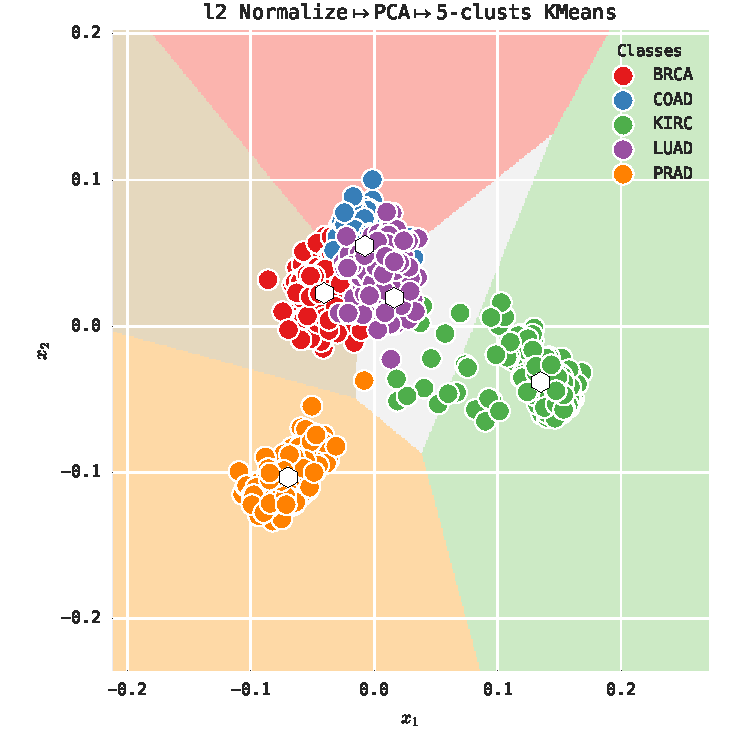
\includegraphics[width=0.3\textwidth]{figures/l2-pca-KMeans_5-clusts.pdf}%
        \label{fig:a}%
    }%
    \hfill%
    \subfloat[]{%
        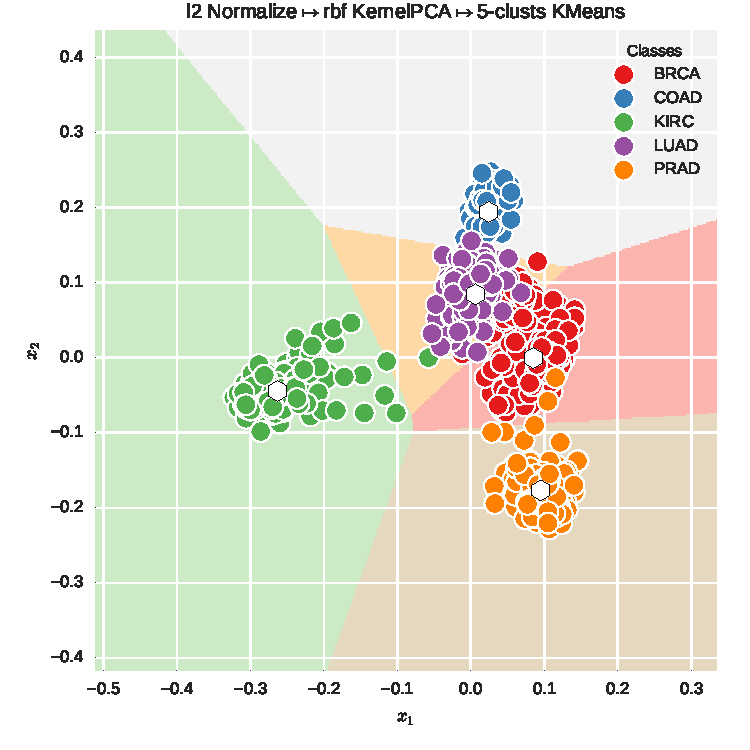
\includegraphics[width=0.3\textwidth]{figures/l2-kpca-KMeans_5-clusts.pdf}%
        \label{fig:b}%
    }%
    \hfill%
    \subfloat[]{%
        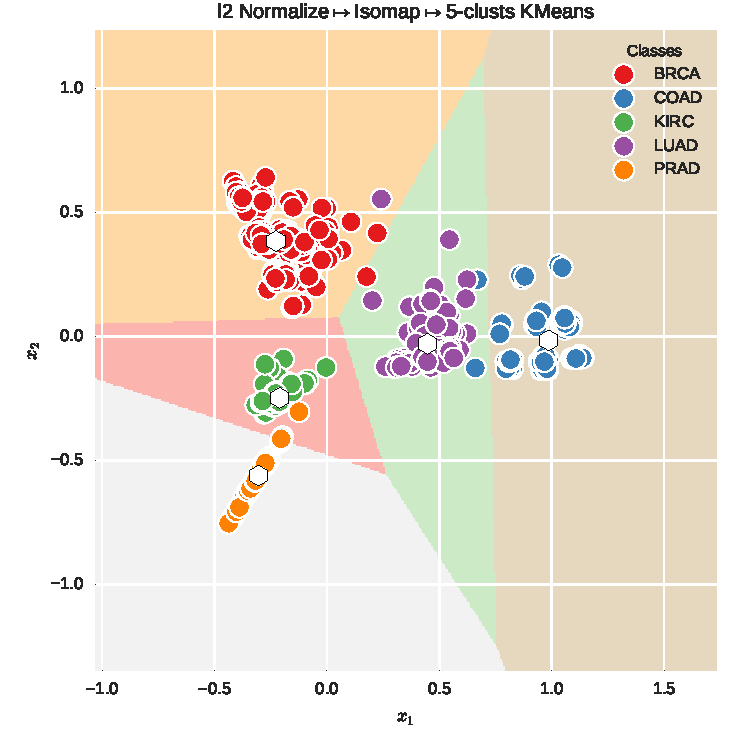
\includegraphics[width=0.3\textwidth]{figures/l2-iso-KMeans_5-clusts.pdf}%
        \label{fig:c}%
    }%
    \caption{\small K-means on three 2D projections of an RNA-Seq data set.}\label{fig:scatter}
\end{figure}


% \acks{Acknowledgements go here.}

\newpage
\bibliography{adenine}

\end{document}
